\documentclass{article}
\usepackage{graphicx}

\begin{document}
    \title{\textbf{ICS Problem Set 9}}
    \maketitle
    \section{\textbf{Problem 9.1}}
    \begin{center}
        \begin{tabular}{| c | c | c | c | c |}
            \hline
            A & B & $C_{in}$ & Sum & $C_{out}$\\
            \hline
            0 & 1 & 0 & 1 & 0\\
            0 & 0 & 0 & 0 & 0\\
            1 & 1 & 0 & 0 & 1\\
            1 & 0 & 0 & 1 & 0\\
            0 & 1 & 1 & 0 & 1\\
            0 & 0 & 1 & 1 & 0\\
            1 & 1 & 1 & 1 & 1\\
            1 & 0 & 1 & 0 & 1\\
            \hline
        \end{tabular}
    \end{center}
    We can derive the DNF and CNF of the Sum and $C_{out}$ from the truth table above.\\
    \\
    For Sum:\\
    DNF:\\
    $(\neg A \land B \land \neg C) \lor (A \land \neg B \land \neg C) \lor (\neg A \land \neg B \land C) \lor (A \land B \land C)$\\
    \\
    CNF:\\
    $(A \lor B \lor C) \land (\neg A \lor \neg B \lor C) \land (A \lor \neg B \lor \neg C) \land (\neg A \lor B \lor \neg C)$\\
    \\
    For $C_{out}$\\
    DNF:\\
    $(A \land B \land \neg C) \lor (\neg A \land B \land C) \lor (A \land B \land C) \lor (A \land \neg B \land C)$\\
    \\
    CNF:\\
    $(A \lor \neg B \lor C) \land (A \lor B \lor C) \land (\neg A \lor B \lor C) \land (A \lor B \lor \neg C)$\\
    \\
    
    \pagebreak
    \ \\
    A Full Adder circuit can be made by using two half adder circuits and a carry bit circuit.\\
    For the first half adder circuit:\\
    \\
    $(A \uparrow (A \uparrow B)) \uparrow (B \uparrow (A \uparrow B))$\\
    \\
    We represent the output of this circuit as $H$ and then pass it into another half adder that takes in $H$ and $C_{in}$ as the input.\\
    For the second half adder circuit:\\
    \\
    $(H \uparrow (H \uparrow C_{in})) \uparrow (C_{in} \uparrow (H \uparrow C_{in}))$\\
    \\
    The carry circuit is then:\\
    \\
    $(A \uparrow B) \uparrow (H \uparrow C_{in})$\\
    \\
    The final circuit can then be represented as:\\
    \\
    \textbf{Sum Circuit:}\\
    \\
    $(((A \uparrow (A \uparrow B)) \uparrow (B \uparrow (A \uparrow B))) \uparrow (((A \uparrow (A \uparrow B)) \uparrow (B \uparrow (A \uparrow B))) \uparrow C_{in})) \uparrow (C_{in} \uparrow (((A \uparrow (A \uparrow B)) \uparrow (B \uparrow (A \uparrow B))) \uparrow C_{in}))$\\
    \\
    \textbf{$C_{out}$ Circuit:}\\
    \\
    $(A \uparrow B) \uparrow (((A \uparrow (A \uparrow B)) \uparrow (B \uparrow (A \uparrow B)) \uparrow C_{in})$\\
    \\
    
    \begin{figure}
    	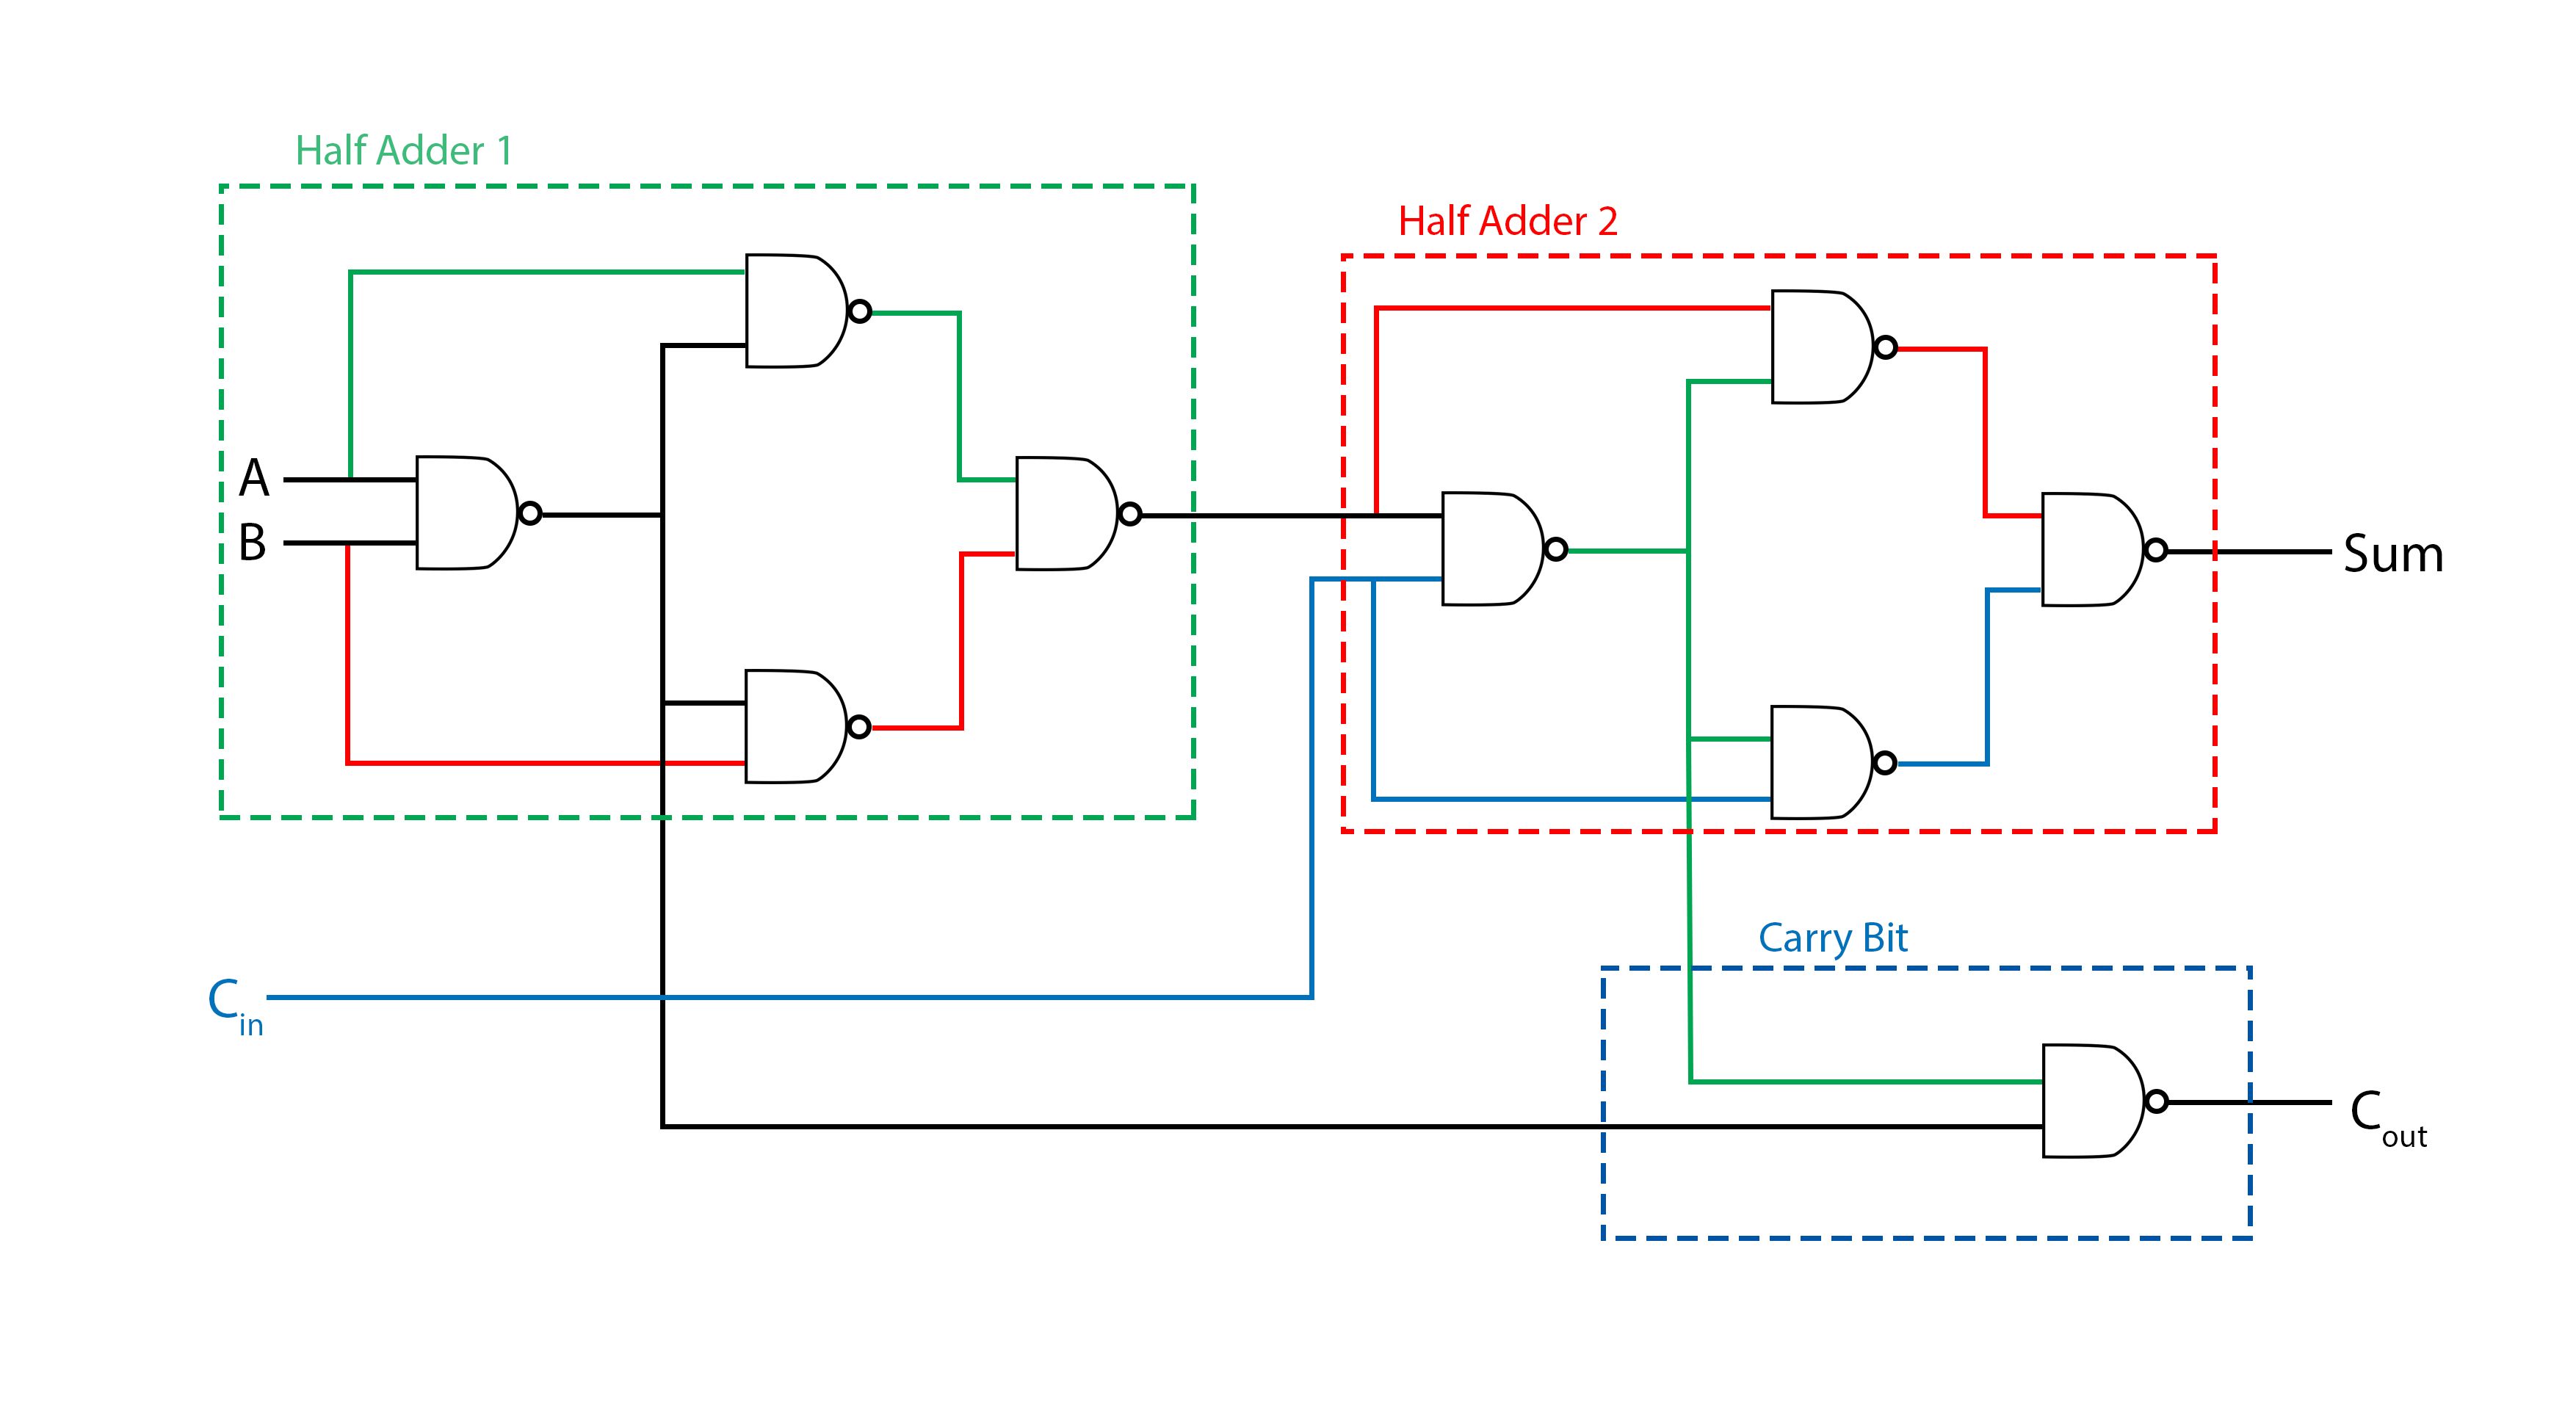
\includegraphics[height=12cm, angle=270]{fulladder2.png}
    	\caption{Full Adder Circuit using NAND gates}
    \end{figure}
	\pagebreak
	
	\section{\textbf{Problem 9.2}}
	\subsection{a}
	Let op be an associative operation with e as the natural element.\\
	Being an associative operator means that:\\
	\\
    $x \  op \  (y \  op \  z) = (x \  op \  y) \ op \  z$\\
    \\
    Now we take a finite list with $n \in N$ elements.\\
    \\
    $xs = [a_1, a_2, ..., a_n]$\\
    \\
    From the given definition of the operator we can derive \textbf{(1)}:\\
    \\
    $\forall p, q, r \in N , p < q < r < n : (a_p \  op \  a_q) \  op \  a_r = (a_p \  op \  (a_q \  op \  a_r)) $\\
    \\
    From the given definition of fold, we can say:\\
    \\
    $foldl \  op \  e \  xs = (((e \  op \  a_1) \  op \  a_2)...\  op \  a_n)$\\
    \\
    Since e is the natural element of the operation, we can write the expression as:\\
    \\
    $foldl \  op \  e \  xs = (((a_1 \  op \  a_2) \  op \  a_3)...\  op \  a_n)$\\
    \\
    From the given definition of foldr, we can say:\\
    \\ 
    $foldr \  op \  e \  xs = (((e \  op \  a_n) \  op \  a_{n-1})...\  op \  a_1)$\\
    \\
    Since e is the natural element of the operation, we can write the expression as:\\
    \\
    $foldr \  op \  e \  xs = (((a_n \  op \  a_{n-1}) \  op \  a_{n-2})...\  op \  a_1)$\\
    \\
    Applying \textbf{(1)} to foldr, we get:\\
    \\
    $foldr \  op \  e \  xs = (((a_1 \  op \  a_2) \  op \  a_3)...\  op \  a_n)$\\
    \\
    $foldr \  op \  e \  xs = foldl \  op \  e \  xs$\\
    \\
    \subsection{b}
    Here op1 and op2 are associative with each other i.e. the precedence of both operations is the same and the order with which they are evaluated does not matter. (As shown in subsection a).
    There exists an element e such that:\\
    \\
    $x \  op1 \  e = e \  op2 \  x$\\
    \\
    Which also means that the following holds:\\
    $e \  op1 \  x = x \  op2 \  e$\\
    \\
    We know:\\
    \\
    $foldl \  op1 \  e \  xs = (((e \  op1 \  a_1) \  op1 \  a_2)...\  op1 \  a_n)$\\
    \\
    But since the order of evaluation of the operators does not matter, we can write it as:\\
    \\
    $foldl \  op1 \  e \  xs = e \  op1 \  (((a_1) \  op1 \  a_2)...\  op1 \  a_n)$\\
    \\
    Again, for foldr:\\
    \\
    $foldr \  op2\  e \  xs = (((a_n \  op2 \  a_{n-1}) \  op2 \  a_{n-2})...\  op2 \  a_1)$\\
    \\
    But since the order of evaluation of the operator does not matter, we can write it as:\\
    \\
    $foldr \  op2 \  e \  xs = (((a_1 \  op2 \  a_2) \  op2 \  a_3)...\  op2 \  a_n) \  op2 \  e$\\
    \\
    From the property of e, we can say:\\
    \\
    $e \  op1 \  (((a_1) \  op1 \  a_2)...\  op1 \  a_n) = (((a_1) \  op2 \  a_2)...\  op2 \  a_n) \  op2 \  e$\\
    \\
    Thus:\\
    \\
    $foldl \  op1 \  e \  xs = foldr \  op2 \  e \  xs$\\
    \\
    \pagebreak
    \subsection{\textbf{c}}
    for the operator op it is given:\\
    \\
    $x \  op' \  y = y \  op \  x$\\
    \\
    We have :\\
    \\
    $xs = [a_1, a_2, ..., a_n], \  n \in N$\\
    \\
    Then, (reverse xs) :\\
    \\
    $xs = [a_n, a_{n-1}, ..., a_1]$\\
    \\
    For foldr:\\
    \\
    $foldr \  op \  a \  xs = (a_1 \  op\ (a_2 \  op\  (... (a_n \  op \  a))))$\\
    \\
    $foldl \  op' \  a \  ( reverse \  xs) = ((((a \  op' \  a_n) ...)\  op' \  a_2) \  op' \  a_1)$\\
    \\
    It is given:\\
    \\
    $x \  op' \  y = y \  op \  x$\\
    \\
    Then it can be said:\\
    \\
    $\forall p, q, r \in N, p < q < r < n :\\ a_p \  op \  (a_q \  op \  a_r) = a_p \  op \  (a_r \  op' \  a_q) = (a_r \  op' \  a_q) \  op' \  a_p$\\
    \\
    Applying this to $foldr \  op \  a \  xs$ we get:\\
    \\
    $foldr \  op \  a \  xs = ((((a \  op' \  a_n) ...)\  op' \  a_2) \  op' \  a_1)$\\
    \\
    $foldr \  op \  a \  xs = foldl \  op' \  a \  ( reverse \  xs)$\\
    \\
\end{document}